% !Rnw weave = knitr
\documentclass[11pt, a4paper]{article}\usepackage[]{graphicx}\usepackage[]{xcolor}
% maxwidth is the original width if it is less than linewidth
% otherwise use linewidth (to make sure the graphics do not exceed the margin)
\makeatletter
\def\maxwidth{ %
  \ifdim\Gin@nat@width>\linewidth
    \linewidth
  \else
    \Gin@nat@width
  \fi
}
\makeatother

\definecolor{fgcolor}{rgb}{0.345, 0.345, 0.345}
\newcommand{\hlnum}[1]{\textcolor[rgb]{0.686,0.059,0.569}{#1}}%
\newcommand{\hlsng}[1]{\textcolor[rgb]{0.192,0.494,0.8}{#1}}%
\newcommand{\hlcom}[1]{\textcolor[rgb]{0.678,0.584,0.686}{\textit{#1}}}%
\newcommand{\hlopt}[1]{\textcolor[rgb]{0,0,0}{#1}}%
\newcommand{\hldef}[1]{\textcolor[rgb]{0.345,0.345,0.345}{#1}}%
\newcommand{\hlkwa}[1]{\textcolor[rgb]{0.161,0.373,0.58}{\textbf{#1}}}%
\newcommand{\hlkwb}[1]{\textcolor[rgb]{0.69,0.353,0.396}{#1}}%
\newcommand{\hlkwc}[1]{\textcolor[rgb]{0.333,0.667,0.333}{#1}}%
\newcommand{\hlkwd}[1]{\textcolor[rgb]{0.737,0.353,0.396}{\textbf{#1}}}%
\let\hlipl\hlkwb

\usepackage{framed}
\makeatletter
\newenvironment{kframe}{%
 \def\at@end@of@kframe{}%
 \ifinner\ifhmode%
  \def\at@end@of@kframe{\end{minipage}}%
  \begin{minipage}{\columnwidth}%
 \fi\fi%
 \def\FrameCommand##1{\hskip\@totalleftmargin \hskip-\fboxsep
 \colorbox{shadecolor}{##1}\hskip-\fboxsep
     % There is no \\@totalrightmargin, so:
     \hskip-\linewidth \hskip-\@totalleftmargin \hskip\columnwidth}%
 \MakeFramed {\advance\hsize-\width
   \@totalleftmargin\z@ \linewidth\hsize
   \@setminipage}}%
 {\par\unskip\endMakeFramed%
 \at@end@of@kframe}
\makeatother

\definecolor{shadecolor}{rgb}{.97, .97, .97}
\definecolor{messagecolor}{rgb}{0, 0, 0}
\definecolor{warningcolor}{rgb}{1, 0, 1}
\definecolor{errorcolor}{rgb}{1, 0, 0}
\newenvironment{knitrout}{}{} % an empty environment to be redefined in TeX

\usepackage{alltt}

% packages
\usepackage[margin=1in]{geometry}
\usepackage{amsmath}
\usepackage{graphicx}
\usepackage{hyperref}
\usepackage{booktabs}
\usepackage{float}

% title page
\title{\textbf{STATS 786: Group Project} \\ Average Monthly Temperatures in Wellington}
\author{
  Group Leader: [palceholder] \\
  Group Members: [Eric Heo], [Dominicus Nararya], [Simon Loh]
}
\date{\today}
\IfFileExists{upquote.sty}{\usepackage{upquote}}{}
\begin{document}

\maketitle

% R Setup Chunk


\tableofcontents
\newpage

\section{Data Cleaning and Exploratory Data Analysis}

The dataset contains average monthly temperatures for Wellington. To prepare the data for modeling, we first formatted the date index and cast the data into a \texttt{tsibble} object. As per the project requirements, we split the data into a training set (all data up to April 2025) and a test set containing the final $h=12$ months (May 2025 to April 2026) to evaluate our models' true predictive performance. 

We also scanned the series for missing values. Because temperature data is heavily driven by the time of year, simple imputation methods like Last Observation Carried Forward (LOCF) or linear interpolation can distort the natural seasonal curve if a gap occurs during a seasonal peak or trough. To determine the best strategy, we plotted multiple imputation techniques against each other. We selected Seasonal Interpolation (\texttt{na\_seadec}), which decomposes the series, interpolates the seasonally adjusted data, and adds the seasonality back in, preserving the natural climate cycles.

\begin{knitrout}
\definecolor{shadecolor}{rgb}{0.969, 0.969, 0.969}\color{fgcolor}\begin{kframe}
\begin{alltt}
\hldef{data} \hlkwb{<-} \hlkwd{read_csv}\hldef{(}\hlsng{"wellington.csv"}\hldef{)} \hlopt{%>%}
  \hlkwd{mutate}\hldef{(}\hlkwc{Date} \hldef{=} \hlkwd{yearmonth}\hldef{(}\hlkwd{paste}\hldef{(Year, Month)))} \hlopt{%>%}
  \hlkwd{select}\hldef{(}\hlopt{-}\hldef{Month,} \hlopt{-}\hldef{Year)} \hlopt{%>%}
  \hlkwd{as_tsibble}\hldef{(}\hlkwc{index} \hldef{= Date)}

\hlcom{# scanning for missing values}
\hlkwd{colSums}\hldef{(}\hlkwd{is.na}\hldef{(data))}
\end{alltt}
\begin{verbatim}
## Temperature        Date 
##           0           0
\end{verbatim}
\begin{alltt}
\hlkwd{scan_gaps}\hldef{(data)}
\end{alltt}
\begin{verbatim}
## # A tsibble: 15 x 1 [1M]
##        Date
##       <mth>
##  1 1993 May
##  2 1993 Jun
##  3 1993 Jul
##  4 1993 Aug
##  5 1993 Sep
##  6 1993 Oct
##  7 1993 Nov
##  8 1993 Dec
##  9 1994 Jan
## 10 1994 Feb
## 11 1994 Mar
## 12 1994 Apr
## 13 1994 May
## 14 1994 Jun
## 15 1994 Jul
\end{verbatim}
\begin{alltt}
\hlcom{# filling implicit gaps in time index}
\hldef{data} \hlkwb{<-} \hldef{data} \hlopt{%>%} \hlkwd{fill_gaps}\hldef{()}

\hlcom{# convert to ts for imputeTS methods}
\hldef{temp_ts} \hlkwb{<-} \hlkwd{ts}\hldef{(data}\hlopt{$}\hldef{Temperature,} \hlkwc{frequency} \hldef{=} \hlnum{12}\hldef{)}

\hlcom{# create comparison dataframe with all methods}
\hldef{comparison} \hlkwb{<-} \hldef{data} \hlopt{%>%}
  \hlkwd{as_tibble}\hldef{()} \hlopt{%>%}
  \hlkwd{mutate}\hldef{(}
    \hlkwc{Original}        \hldef{= Temperature,}
    \hlkwc{LOCF}            \hldef{=} \hlkwd{as.numeric}\hldef{(}\hlkwd{na.locf}\hldef{(temp_ts,} \hlkwc{na.rm} \hldef{=} \hlnum{FALSE}\hldef{)),}
    \hlkwc{NOCB}            \hldef{=} \hlkwd{as.numeric}\hldef{(}\hlkwd{na.locf}\hldef{(temp_ts,} \hlkwc{fromLast} \hldef{=} \hlnum{TRUE}\hldef{,} \hlkwc{na.rm} \hldef{=} \hlnum{FALSE}\hldef{)),}
    \hlkwc{Linear}          \hldef{=} \hlkwd{as.numeric}\hldef{(}\hlkwd{na_interpolation}\hldef{(temp_ts,} \hlkwc{option} \hldef{=} \hlsng{"linear"}\hldef{)),}
    \hlkwc{Spline}          \hldef{=} \hlkwd{as.numeric}\hldef{(}\hlkwd{na_interpolation}\hldef{(temp_ts,} \hlkwc{option} \hldef{=} \hlsng{"spline"}\hldef{)),}
    \hlkwc{Seasonal}        \hldef{=} \hlkwd{as.numeric}\hldef{(}\hlkwd{na_seadec}\hldef{(temp_ts,} \hlkwc{algorithm} \hldef{=} \hlsng{"interpolation"}\hldef{))}
  \hldef{)} \hlopt{%>%}
  \hlkwd{select}\hldef{(Date, Original, LOCF, NOCB, Linear, Spline, Seasonal)} \hlopt{%>%}
  \hlkwd{pivot_longer}\hldef{(}\hlopt{-}\hldef{Date,} \hlkwc{names_to} \hldef{=} \hlsng{"Method"}\hldef{,} \hlkwc{values_to} \hldef{=} \hlsng{"Temperature"}\hldef{)}

\hldef{comparison} \hlopt{%>%}
  \hlkwd{mutate}\hldef{(}\hlkwc{Method} \hldef{=} \hlkwd{factor}\hldef{(Method,} \hlkwc{levels} \hldef{=} \hlkwd{c}\hldef{(}\hlsng{"Original"}\hldef{,} \hlsng{"LOCF"}\hldef{,} \hlsng{"NOCB"}\hldef{,}
                                             \hlsng{"Linear"}\hldef{,} \hlsng{"Spline"}\hldef{,} \hlsng{"Seasonal"}\hldef{)))} \hlopt{%>%}
  \hlkwd{ggplot}\hldef{(}\hlkwd{aes}\hldef{(}\hlkwc{x} \hldef{= Date,} \hlkwc{y} \hldef{= Temperature))} \hlopt{+}
  \hlkwd{geom_line}\hldef{(}\hlkwc{linewidth} \hldef{=} \hlnum{0.3}\hldef{)} \hlopt{+}
  \hlkwd{facet_wrap}\hldef{(}\hlopt{~} \hldef{Method,} \hlkwc{ncol} \hldef{=} \hlnum{1}\hldef{)} \hlopt{+}
  \hlkwd{labs}\hldef{(}\hlkwc{title} \hldef{=} \hlsng{"Wellington Monthly Temperature — Interpolation Method Comparison"}\hldef{,}
       \hlkwc{y} \hldef{=} \hlsng{"Temperature (°C)"}\hldef{,} \hlkwc{x} \hldef{=} \hlsng{"Date"}\hldef{)} \hlopt{+}
  \hlkwd{theme_minimal}\hldef{()} \hlopt{+}
  \hlkwd{theme}\hldef{(}\hlkwc{strip.text} \hldef{=} \hlkwd{element_text}\hldef{(}\hlkwc{face} \hldef{=} \hlsng{"bold"}\hldef{))}
\end{alltt}
\end{kframe}\begin{figure}[H]

{\centering 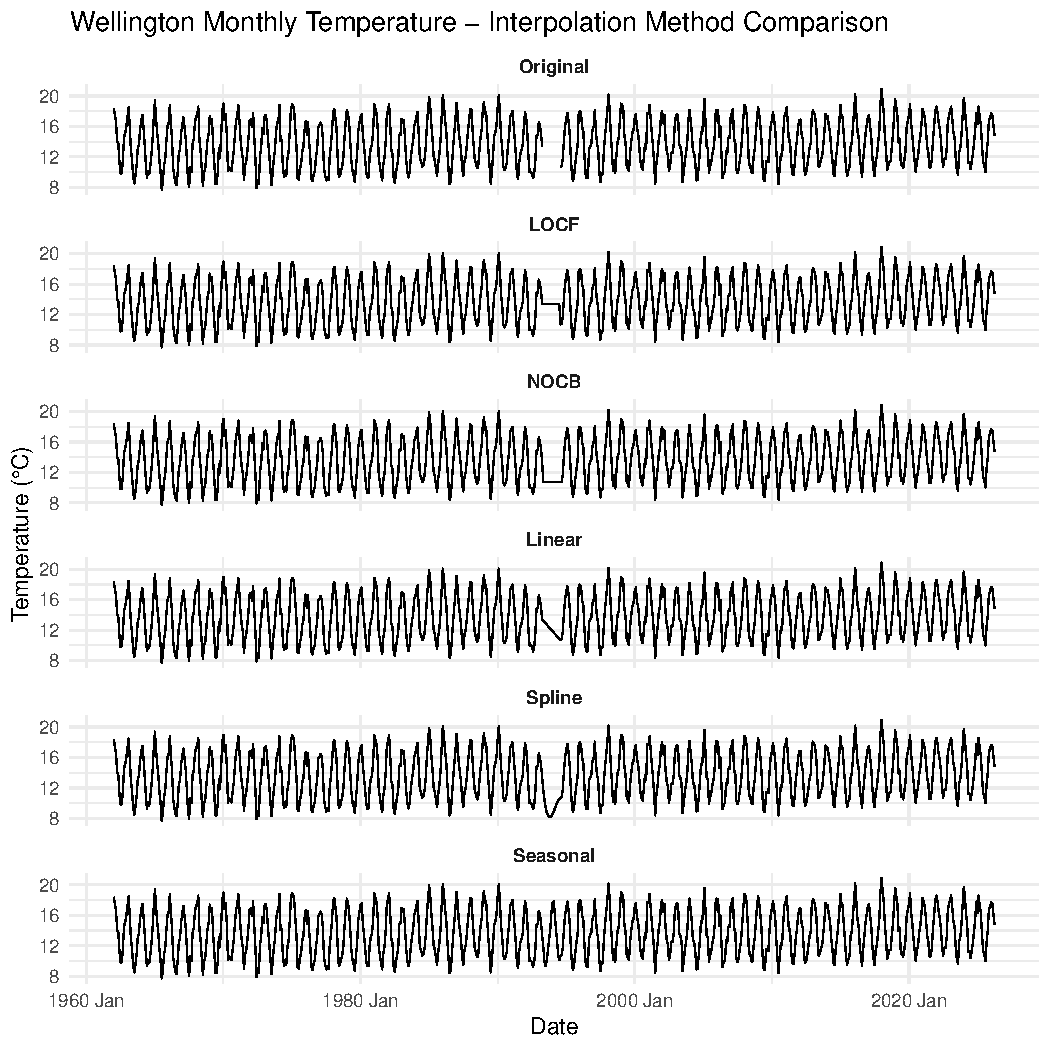
\includegraphics[width=1\linewidth]{figure/data-cleaning-1} 

}

\caption[Comparison of Missing Value Imputation Methods]{Comparison of Missing Value Imputation Methods}\label{fig:data-cleaning}
\end{figure}

\begin{kframe}\begin{alltt}
\hlcom{# apply chosen seasonal imputation}
\hldef{data} \hlkwb{<-} \hldef{data} \hlopt{%>%}
  \hlkwd{mutate}\hldef{(}\hlkwc{Temperature} \hldef{=} \hlkwd{na_seadec}\hldef{(Temperature,} \hlkwc{algorithm} \hldef{=} \hlsng{"interpolation"}\hldef{,} \hlkwd{frequency}\hldef{(}\hlnum{12}\hldef{)))} \hlopt{%>%}
  \hlkwd{mutate}\hldef{(}\hlkwc{Temperature} \hldef{=} \hlkwd{as.numeric}\hldef{(Temperature))}

\hlcom{# creating training + test sets}
\hldef{training} \hlkwb{<-} \hldef{data} \hlopt{%>%}
  \hlkwd{filter}\hldef{(Date} \hlopt{<=} \hlkwd{yearmonth}\hldef{(}\hlsng{"2025 April"}\hldef{))}

\hldef{test} \hlkwb{<-} \hldef{data} \hlopt{%>%}
  \hlkwd{filter}\hldef{(Date} \hlopt{>} \hlkwd{yearmonth}\hldef{(}\hlsng{"2025 April"}\hldef{))}
\end{alltt}
\end{kframe}
\end{knitrout}

\subsection{Visualizing the Time Series}
To understand the underlying behavior of Wellington's temperatures, we produced a standard time plot, a seasonal subseries plot, and an STL decomposition.

\begin{knitrout}
\definecolor{shadecolor}{rgb}{0.969, 0.969, 0.969}\color{fgcolor}\begin{kframe}
\begin{alltt}
\hlcom{# standard time plot}
\hldef{data} \hlopt{%>%}
  \hlkwd{autoplot}\hldef{(Temperature)} \hlopt{+}
  \hlkwd{labs}\hldef{(}\hlkwc{title} \hldef{=} \hlsng{"Wellington Monthly Temperature"}\hldef{,}
       \hlkwc{y} \hldef{=} \hlsng{"Temperature (°C)"}\hldef{,}
       \hlkwc{x} \hldef{=} \hlsng{"Date"}\hldef{)} \hlopt{+}
  \hlkwd{theme_minimal}\hldef{()}

\hlcom{# seasonal subseries plot}
\hldef{data} \hlopt{%>%}
  \hlkwd{gg_subseries}\hldef{(Temperature)} \hlopt{+}
  \hlkwd{labs}\hldef{(}\hlkwc{title} \hldef{=} \hlsng{"Wellington Temperature Seasonal Subseries"}\hldef{,}
       \hlkwc{y} \hldef{=} \hlsng{"Temperature (°C)"}\hldef{,}
       \hlkwc{x} \hldef{=} \hlsng{"Month"}\hldef{)} \hlopt{+}
  \hlkwd{theme_minimal}\hldef{()}

\hlcom{# STL decomp}
\hldef{data} \hlopt{%>%}
  \hlkwd{model}\hldef{(}\hlkwd{STL}\hldef{(Temperature} \hlopt{~} \hlkwd{trend}\hldef{()} \hlopt{+} \hlkwd{season}\hldef{(}\hlkwc{window} \hldef{=} \hlsng{"periodic"}\hldef{)))} \hlopt{%>%}
  \hlkwd{components}\hldef{()} \hlopt{%>%}
  \hlkwd{autoplot}\hldef{()} \hlopt{+}
  \hlkwd{labs}\hldef{(}\hlkwc{title} \hldef{=} \hlsng{"STL Decomposition of Wellington Temperature"}\hldef{)} \hlopt{+}
  \hlkwd{theme_minimal}\hldef{()}
\end{alltt}
\end{kframe}

{\centering 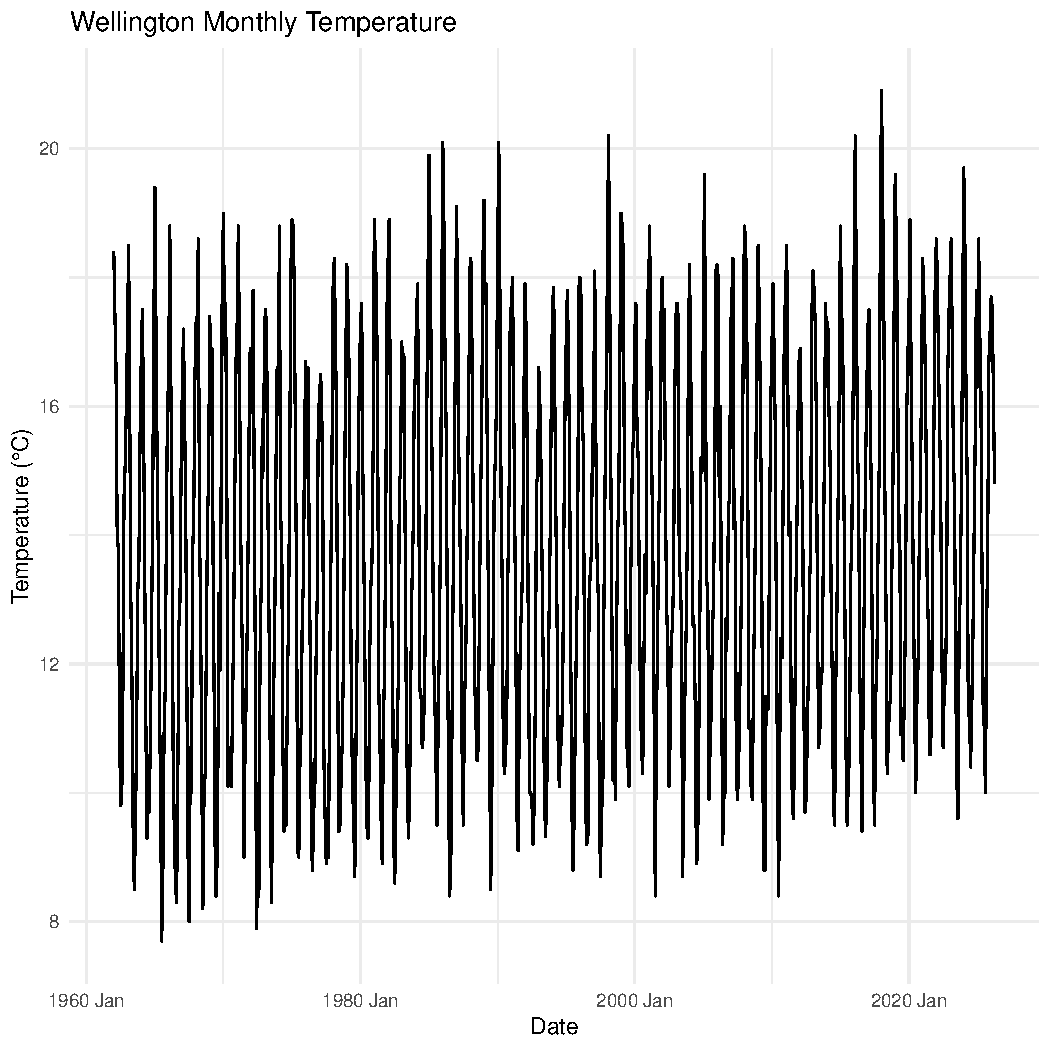
\includegraphics[width=1\linewidth]{figure/eda-plots-1} 
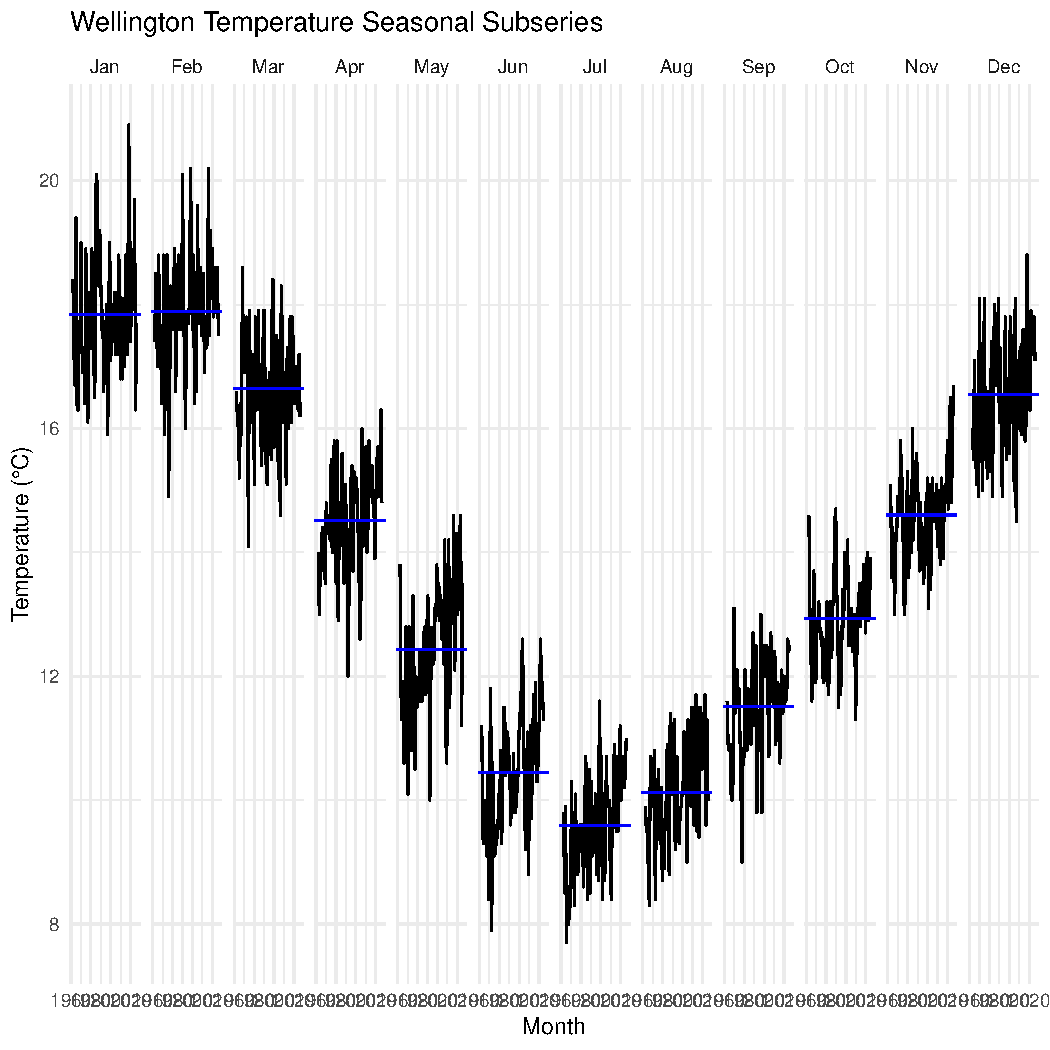
\includegraphics[width=1\linewidth]{figure/eda-plots-2} 
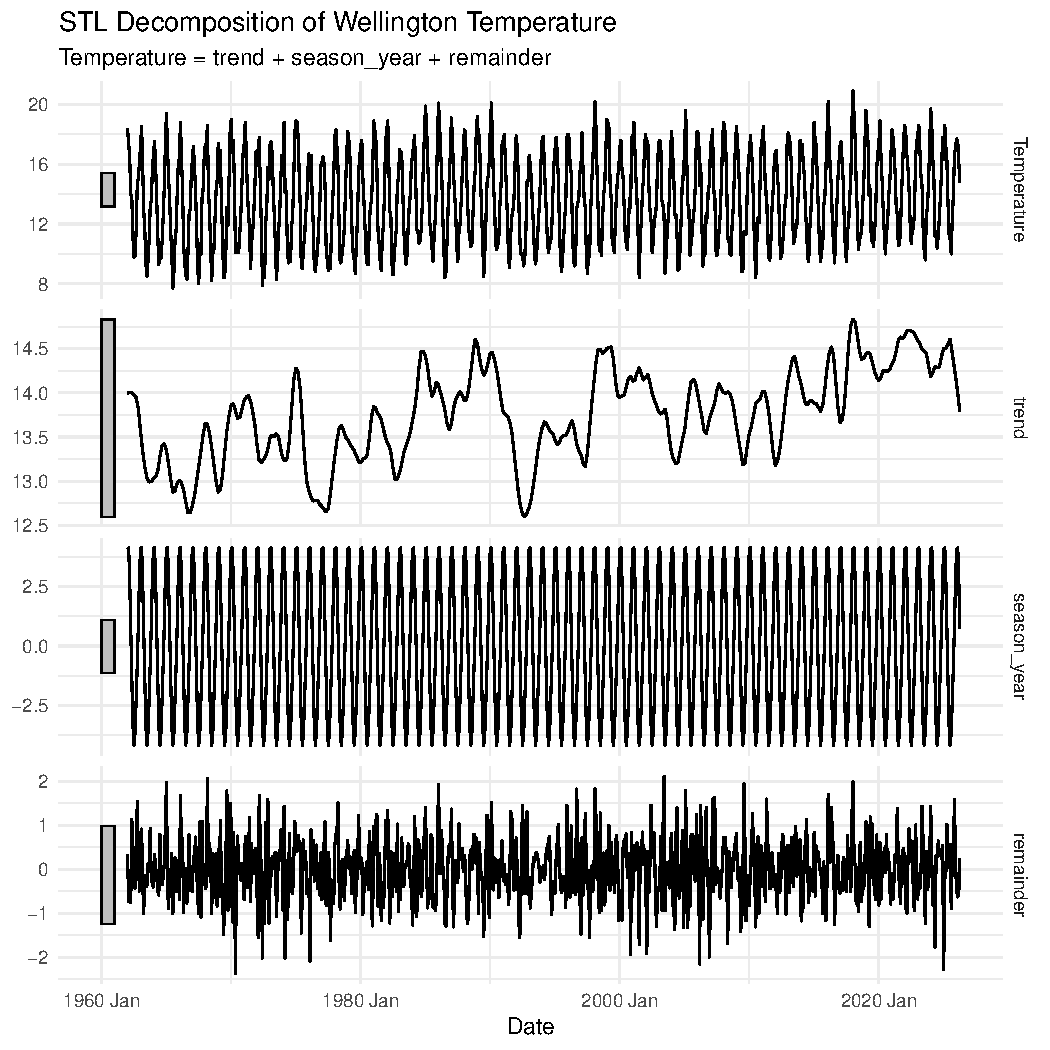
\includegraphics[width=1\linewidth]{figure/eda-plots-3} 

}


\end{knitrout}

\textbf{Observed Features:}
palceholder ghaksfsgjdklnbkjdnkjsjkgserf

\section{ETS Models}

The trend component in the STL decomposition shows that there is a slight upward trend with Temperature increasing over time with peaks and troughs of 14.0 and 12.5 C in the 1960's to 15.0 and 13.5 C in the 2010's. Three trend specifications were considered no trend (N), additive trend (A), and damped additive trend (Ad).

The remainder component shows roughly constant variance throughout the whole time series from 1960 to 2025 meaning there is no heteroscedacity. This means that additive errors (A) are appropriate, so we will not include multiplicative error models. 

The seasonal component shows highly stable yearly annual cycle that remains unchanged over the whole time series. As the magnitude of seasonal fluctuations does not vary, additive seasonality (A) is appropriate. We will not consider multiplicative seasonality.

As such the following models were shortlisted:
ETS(A,N,A), ETS(A,A,A), and ETS(A,Ad,A).

\begin{knitrout}
\definecolor{shadecolor}{rgb}{0.969, 0.969, 0.969}\color{fgcolor}\begin{kframe}
\begin{alltt}
\hldef{fit} \hlkwb{<-} \hldef{training} \hlopt{%>%}
  \hlkwd{model}\hldef{(}
    \hlkwc{ANA}  \hldef{=} \hlkwd{ETS}\hldef{(Temperature} \hlopt{~} \hlkwd{error}\hldef{(}\hlsng{"A"}\hldef{)} \hlopt{+} \hlkwd{trend}\hldef{(}\hlsng{"N"}\hldef{)} \hlopt{+} \hlkwd{season}\hldef{(}\hlsng{"A"}\hldef{)),}
    \hlkwc{AAA}  \hldef{=} \hlkwd{ETS}\hldef{(Temperature} \hlopt{~} \hlkwd{error}\hldef{(}\hlsng{"A"}\hldef{)} \hlopt{+} \hlkwd{trend}\hldef{(}\hlsng{"A"}\hldef{)} \hlopt{+} \hlkwd{season}\hldef{(}\hlsng{"A"}\hldef{)),}
    \hlkwc{AAdA} \hldef{=} \hlkwd{ETS}\hldef{(Temperature} \hlopt{~} \hlkwd{error}\hldef{(}\hlsng{"A"}\hldef{)} \hlopt{+} \hlkwd{trend}\hldef{(}\hlsng{"Ad"}\hldef{)} \hlopt{+} \hlkwd{season}\hldef{(}\hlsng{"A"}\hldef{)),}
    \hlkwc{auto} \hldef{=} \hlkwd{ETS}\hldef{(Temperature)}
  \hldef{)}

\hldef{fit} \hlopt{%>%} \hlkwd{select}\hldef{(auto)} \hlopt{%>%} \hlkwd{report}\hldef{()}
\end{alltt}
\begin{verbatim}
## Series: Temperature 
## Model: ETS(A,N,A) 
##   Smoothing parameters:
##     alpha = 0.125848 
##     gamma = 0.0001000595 
## 
##   Initial states:
##      l[0]     s[0]     s[-1]      s[-2]     s[-3]     s[-4]     s[-5]     s[-6]
##  13.75272 2.827684 0.8530713 -0.8283216 -2.208586 -3.629442 -4.199804 -3.342363
##      s[-7]     s[-8]    s[-9]  s[-10]   s[-11]
##  -1.297429 0.7641372 2.861139 4.11656 4.083353
## 
##   sigma^2:  0.7357
## 
##      AIC     AICc      BIC 
## 4823.964 4824.610 4893.464
\end{verbatim}
\begin{alltt}
\hlkwd{glance}\hldef{(fit)} \hlopt{%>%}
  \hlkwd{select}\hldef{(.model, AIC, AICc, BIC)} \hlopt{%>%}
  \hlkwd{arrange}\hldef{(AICc)}
\end{alltt}
\begin{verbatim}
## # A tibble: 4 x 4
##   .model   AIC  AICc   BIC
##   <chr>  <dbl> <dbl> <dbl>
## 1 ANA    4824. 4825. 4893.
## 2 auto   4824. 4825. 4893.
## 3 AAdA   4830. 4831. 4914.
## 4 AAA    4834. 4835. 4912.
\end{verbatim}
\end{kframe}
\end{knitrout}

The ETS(A,N,A) model will likely have the best predictive ability as it has the lowest AICc (manually) and was also the best model automatically selected. This suggests that even though there is a slight increasing trend of temperature in the STL decomposition, the trend component does not improve out-of-sample predictive ability. 

The fitted ETS(A,N,A) model equations are as follows:

\[
y_t = \ell_{t-1} + s_{t-12} + \varepsilon_t
\]

\[
\ell_t = \ell_{t-1} + 0.1258\varepsilon_t
\]

\[
s_t = s_{t-12} + 0.0001\varepsilon_t
\]

where $\varepsilon_t \sim \mathrm{NID}(0,\ 0.7357)$ and $\ell_0 = 13.7527$.

\section{ARIMA Models}

\subsection{Transformations/ Differencing Required?}

\begin{knitrout}
\definecolor{shadecolor}{rgb}{0.969, 0.969, 0.969}\color{fgcolor}\begin{kframe}
\begin{alltt}
\hlcom{# 1. Determine Required Differencing}
\hlcom{# Check how many seasonal differences are required}
\hldef{training} \hlopt{%>%}
  \hlkwd{features}\hldef{(Temperature, unitroot_nsdiffs)}
\end{alltt}
\begin{verbatim}
## # A tibble: 1 x 1
##   nsdiffs
##     <int>
## 1       1
\end{verbatim}
\begin{alltt}
\hlcom{# Check how many first differences are required AFTER a seasonal difference}
\hldef{training} \hlopt{%>%}
  \hlkwd{mutate}\hldef{(}\hlkwc{diff_temp} \hldef{=} \hlkwd{difference}\hldef{(Temperature,} \hlnum{12}\hldef{))} \hlopt{%>%}
  \hlkwd{features}\hldef{(diff_temp, unitroot_ndiffs)}
\end{alltt}
\begin{verbatim}
## # A tibble: 1 x 1
##   ndiffs
##    <int>
## 1      0
\end{verbatim}
\begin{alltt}
\hlcom{# 2. Manual Model Identification}
\hlcom{# Plot the differenced data alongside its ACF and PACF.}
\hldef{training} \hlopt{%>%}
  \hlkwd{gg_tsdisplay}\hldef{(}\hlkwd{difference}\hldef{(Temperature,} \hlnum{12}\hldef{),} \hlkwc{plot_type} \hldef{=} \hlsng{"partial"}\hldef{,} \hlkwc{lag_max} \hldef{=} \hlnum{36}\hldef{)} \hlopt{+}
  \hlkwd{labs}\hldef{(}\hlkwc{title} \hldef{=} \hlsng{"Seasonally Differenced Temperature"}\hldef{)}
\end{alltt}
\end{kframe}

{\centering 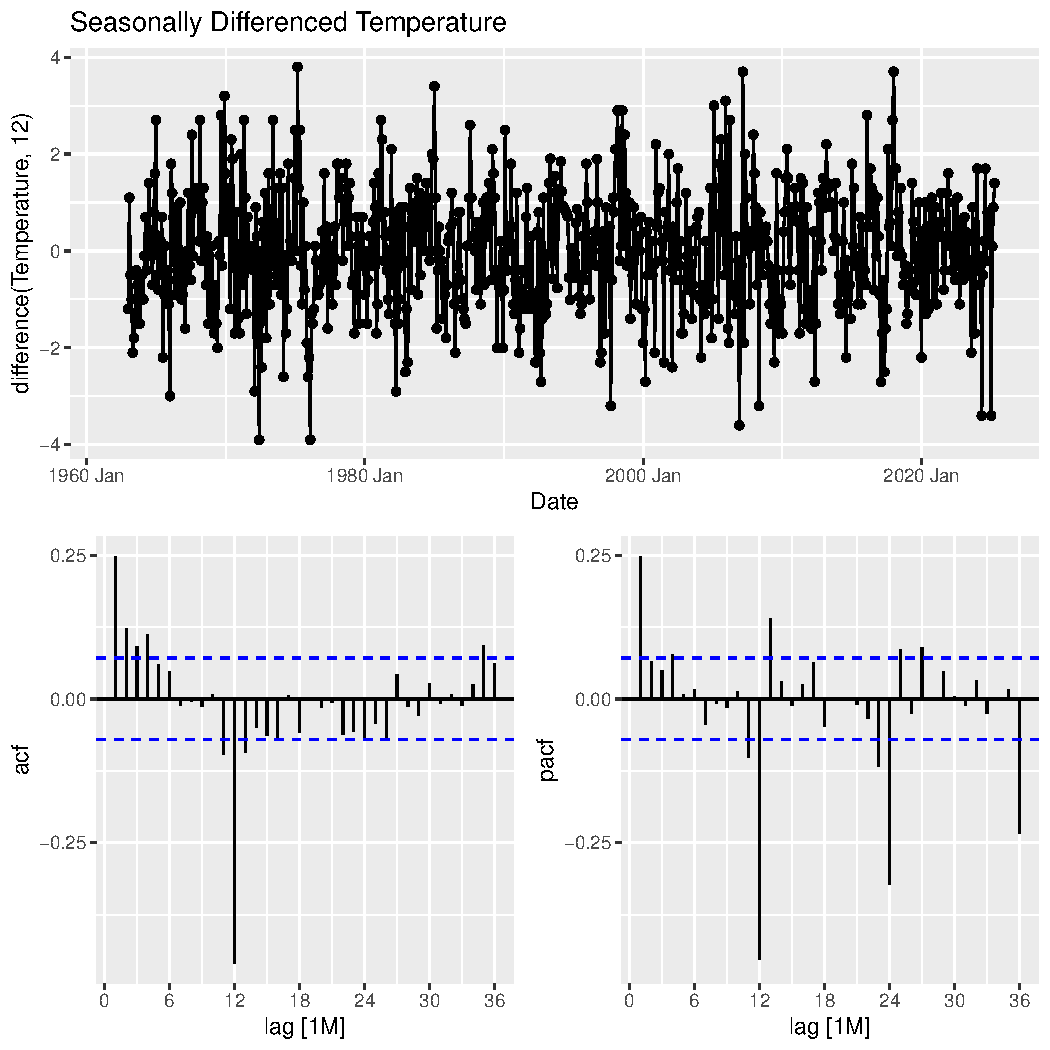
\includegraphics[width=1\linewidth]{figure/arima-models-transformations-1} 

}


\end{knitrout}

1. Transformations (Variance Stabilization) transformations help to stabilize the variance of a time series. In our R code, we did not apply any transformations (such as a logarithm or Box-Cox). This is because the seasonal fluctuations in temperature data typically have a constant variance over time. For ARIMA models, our primary requirement is instead to stabilize the mean of the time series. 

2. Differencing (Mean Stabilization)To stabilize the mean and achieve stationarity, we use differencing. Differencing can be helpful to remove changes in the level of a time series, which eliminates (or reduces) trend and seasonality.In this specific model, we applied one seasonal difference and zero first differences.The Seasonal Difference: A seasonal difference is the difference between an observation and the previous observation from the same season. Because we are dealing with monthly temperature data, our seasonal period is $m=12$. 

\subsection{Methodology}

\begin{knitrout}
\definecolor{shadecolor}{rgb}{0.969, 0.969, 0.969}\color{fgcolor}\begin{kframe}
\begin{alltt}
\hlcom{# 3. Fit Candidate ARIMA Models}

\hldef{fit_arima} \hlkwb{<-} \hldef{training} \hlopt{%>%}
  \hlkwd{model}\hldef{(}
    \hlkwc{manual_1} \hldef{=} \hlkwd{ARIMA}\hldef{(Temperature} \hlopt{~} \hlkwd{pdq}\hldef{(}\hlnum{0}\hldef{,}\hlnum{0}\hldef{,}\hlnum{1}\hldef{)} \hlopt{+} \hlkwd{PDQ}\hldef{(}\hlnum{0}\hldef{,}\hlnum{1}\hldef{,}\hlnum{1}\hldef{)),}
    \hlkwc{manual_2} \hldef{=} \hlkwd{ARIMA}\hldef{(Temperature} \hlopt{~} \hlkwd{pdq}\hldef{(}\hlnum{1}\hldef{,}\hlnum{0}\hldef{,}\hlnum{0}\hldef{)} \hlopt{+} \hlkwd{PDQ}\hldef{(}\hlnum{0}\hldef{,}\hlnum{1}\hldef{,}\hlnum{1}\hldef{)),}

    \hlkwc{auto_stepwise} \hldef{=} \hlkwd{ARIMA}\hldef{(Temperature),}

    \hlkwc{auto_search} \hldef{=} \hlkwd{ARIMA}\hldef{(Temperature,} \hlkwc{stepwise} \hldef{=} \hlnum{FALSE}\hldef{)}
  \hldef{)}

\hldef{fit_arima} \hlopt{%>%} \hlkwd{select}\hldef{(auto_search)} \hlopt{%>%} \hlkwd{report}\hldef{()}
\end{alltt}
\begin{verbatim}
## Series: Temperature 
## Model: ARIMA(2,0,1)(2,1,0)[12] 
## 
## Coefficients:
##          ar1      ar2     ma1     sar1     sar2
##       0.9383  -0.0806  -0.716  -0.6768  -0.3743
## s.e.  0.1894   0.0968   0.160   0.0354   0.0355
## 
## sigma^2 estimated as 0.9359:  log likelihood=-1037.54
## AIC=2087.08   AICc=2087.2   BIC=2114.79
\end{verbatim}
\begin{alltt}
\hlcom{# Compare models wit AICc }
\hlkwd{glance}\hldef{(fit_arima)} \hlopt{%>%}
  \hlkwd{arrange}\hldef{(AICc)} \hlopt{%>%}
  \hlkwd{select}\hldef{(.model}\hlopt{:}\hldef{BIC)}
\end{alltt}
\begin{verbatim}
## # A tibble: 4 x 6
##   .model        sigma2 log_lik   AIC  AICc   BIC
##   <chr>          <dbl>   <dbl> <dbl> <dbl> <dbl>
## 1 manual_2       0.819   -986. 1950. 1950. 1968.
## 2 manual_1       0.845   -997. 1972. 1972. 1990.
## 3 auto_search    0.936  -1038. 2087. 2087. 2115.
## 4 auto_stepwise  1.09   -1092. 2196. 2196. 2223.
\end{verbatim}
\begin{alltt}
\hldef{best_arima} \hlkwb{<-} \hldef{fit_arima} \hlopt{%>%} \hlkwd{select}\hldef{(manual_2)}

\hldef{best_arima} \hlopt{%>%} \hlkwd{report}\hldef{()}
\end{alltt}
\begin{verbatim}
## Series: Temperature 
## Model: ARIMA(1,0,0)(0,1,1)[12] w/ drift 
## 
## Coefficients:
##          ar1     sma1  constant
##       0.3173  -0.8785    0.0085
## s.e.  0.0348   0.0179    0.0044
## 
## sigma^2 estimated as 0.8191:  log likelihood=-985.73
## AIC=1950.01   AICc=1950.06   BIC=1968.48
\end{verbatim}
\end{kframe}
\end{knitrout}

Methodology: we shortlist candidate models using both manual inspection and automated algorithms, evaluating them based on the Corrected Akaike's Information Criterion (AICc).  

1. Manual Selection Plot the Autocorrelation Function (ACF) and Partial Autocorrelation Function (PACF) of the appropriately differenced data.  Examine the non-seasonal lags to identify the non-seasonal AR(p) and MA(q) orders. For example, if the ACF tails off and the PACF cuts off after lag p, it suggests an AR(p) model. If the ACF cuts off after lag q and the PACF tails off, it suggests an MA(q) model.  Examine the seasonal lags to identify the seasonal AR(P) and MA(Q) orders .  Fit these chosen models using the ARIMA() function.2. Automatic Selection Stepwise Algorithm: The ARIMA() function in the fable package automatically finds the best ARIMA model by default. It uses a stepwise algorithm to efficiently traverse the model space and selects the model with the lowest AICc.  Exhaustive Search: By setting stepwise = FALSE and approximation = FALSE, the function will search a much larger set of models, which takes longer but can sometimes find a better fitting model than the stepwise approach.  

3. Model Evaluation Check the residuals of your shortlisted models. The residuals should look like white noise. Use \texttt{gg\_tsresiduals()} to visually inspect the ACF of the residuals and perform a Ljung-Box test to ensure they are uncorrelated. 

The manual candidate ARIMA(1,0,0)(0,1,1) with drift was selected as the best model based on the lowest AICc of 1950.06, outperforming both automatic procedures by a substantial margin. The stepwise algorithm performed poorly, and the exhaustive search selected an overly complex ARIMA(2,0,1)(2,1,0) model with a AICc of 137 relative to the best model, a clear sign of overfitting on the training set. This result illustrates that automatic model selection is not always superior to theory-driven manual specification; the ACF and PACF of the seasonally differenced series clearly indicated AR(1) non-seasonal structure and SMA(1) seasonal structure, and the model built directly from those patterns generalised best.

\subsection{Backshift Notation}

\[
(1 - 0.3173\,B)(1 - B^{12})\,y_t 
= 0.0085 + (1 - 0.8785\,B^{12})\,\varepsilon_t
\]
where $\varepsilon_t \sim \mathrm{NID}(0,\ 0.8191)$.

\section{Dynamic Regression Models}

\subsection{Dynamic Regression Explanation}
When we build a standard multiple linear regression model, we have to assume that our errors (the residuals) are not autocorrelated; otherwise, our forecasts become inefficient and our statistical tests become unreliable. In time series data, this assumption is almost always violated because data points collected sequentially are naturally correlated with one another. Dynamic regression addresses this problem by, actively modelling the autocorrelation in the errors using an ARIMA process instead of hoping our errors are random white noise. 

We can think of a dynamic regression model as having two parts:
\begin{enumerate}
    \item \textbf{The Deterministic Part:} The standard regression equation where we predict our target using explanatory variables (like a linear trend, Fourier terms for seasonality, or dummy variables for outlier spikes).
    \item \textbf{The Stochastic Part:} An ARIMA model fitted to the residuals of that regression to capture the remaining time-dependent patterns.
\end{enumerate}

Mathematically, it looks like this:
$$y_t = \beta_0 + \beta_1 x_{1,t} + \dots + \beta_k x_{k,t} + \eta_t$$
Where $y_t$ is our observation, the $\beta$ terms are our regression coefficients, and $\eta_t$ is an ARIMA error term.

\subsection{Model Exploration and Selection}
To capture the monthly seasonality of Wellington's temperatures, we will use a Fourier series (harmonic regression) instead of seasonal dummy variables, as it is highly effective for periodic functions. Because we have monthly data ($m=12$), the maximum number of Fourier pairs $K$ we can include is $m/2 = 6$. 

We will fit models from K=1 to K=6, alongside a linear trend.

\begin{knitrout}
\definecolor{shadecolor}{rgb}{0.969, 0.969, 0.969}\color{fgcolor}\begin{kframe}
\begin{alltt}
\hlcom{# The ARIMA() function will automatically handle ARIMA error fitting procedure}
\hldef{fit_dynamic} \hlkwb{<-} \hldef{training} \hlopt{%>%}
  \hlkwd{model}\hldef{(}
    \hlkwc{K1} \hldef{=} \hlkwd{ARIMA}\hldef{(Temperature} \hlopt{~} \hlkwd{trend}\hldef{()} \hlopt{+} \hlkwd{fourier}\hldef{(}\hlkwc{K} \hldef{=} \hlnum{1}\hldef{)),}
    \hlkwc{K2} \hldef{=} \hlkwd{ARIMA}\hldef{(Temperature} \hlopt{~} \hlkwd{trend}\hldef{()} \hlopt{+} \hlkwd{fourier}\hldef{(}\hlkwc{K} \hldef{=} \hlnum{2}\hldef{)),}
    \hlkwc{K3} \hldef{=} \hlkwd{ARIMA}\hldef{(Temperature} \hlopt{~} \hlkwd{trend}\hldef{()} \hlopt{+} \hlkwd{fourier}\hldef{(}\hlkwc{K} \hldef{=} \hlnum{3}\hldef{)),}
    \hlkwc{K4} \hldef{=} \hlkwd{ARIMA}\hldef{(Temperature} \hlopt{~} \hlkwd{trend}\hldef{()} \hlopt{+} \hlkwd{fourier}\hldef{(}\hlkwc{K} \hldef{=} \hlnum{4}\hldef{)),}
    \hlkwc{K5} \hldef{=} \hlkwd{ARIMA}\hldef{(Temperature} \hlopt{~} \hlkwd{trend}\hldef{()} \hlopt{+} \hlkwd{fourier}\hldef{(}\hlkwc{K} \hldef{=} \hlnum{5}\hldef{)),}
    \hlkwc{K6} \hldef{=} \hlkwd{ARIMA}\hldef{(Temperature} \hlopt{~} \hlkwd{trend}\hldef{()} \hlopt{+} \hlkwd{fourier}\hldef{(}\hlkwc{K} \hldef{=} \hlnum{6}\hldef{))}
  \hldef{)}

\hlkwd{glance}\hldef{(fit_dynamic)} \hlopt{%>%}
  \hlkwd{select}\hldef{(.model, AIC, AICc, BIC)} \hlopt{%>%}
  \hlkwd{arrange}\hldef{(AICc)}
\end{alltt}
\begin{verbatim}
## # A tibble: 6 x 4
##   .model   AIC  AICc   BIC
##   <chr>  <dbl> <dbl> <dbl>
## 1 K3     1893. 1894. 1958.
## 2 K4     1895. 1896. 1969.
## 3 K5     1898. 1899. 1981.
## 4 K6     1900. 1901. 1988.
## 5 K2     1905. 1906. 1952.
## 6 K1     1950. 1950. 1992.
\end{verbatim}
\end{kframe}
\end{knitrout}

We evaluated dynamic regression models ranging from K=1 to K=6. While K=2 provided the lowest BIC, we will select K=3 model for our final forecasts as it yielded the lowest AICc (1893.659), which is the preferred metric for optimising predictive forecasting performance.

\begin{knitrout}
\definecolor{shadecolor}{rgb}{0.969, 0.969, 0.969}\color{fgcolor}\begin{kframe}
\begin{alltt}
\hldef{best_dynamic} \hlkwb{<-} \hldef{fit_dynamic} \hlopt{%>%} \hlkwd{select}\hldef{(K3)}

\hlcom{# get coeffs}
\hldef{dynamic_coefs} \hlkwb{<-} \hlkwd{tidy}\hldef{(best_dynamic)}

\hlcom{# isolate trend() component}
\hldef{trend_component} \hlkwb{<-} \hldef{dynamic_coefs} \hlopt{%>%} \hlkwd{filter}\hldef{(term} \hlopt{==} \hlsng{"trend()"}\hldef{)}

\hlcom{# compute 95% CI for monthly slope}
\hldef{slope} \hlkwb{<-} \hldef{trend_component}\hlopt{$}\hldef{estimate}
\hldef{std_error} \hlkwb{<-} \hldef{trend_component}\hlopt{$}\hldef{std.error}
\hldef{z_val} \hlkwb{<-} \hlnum{1.96}

\hldef{ci_lower} \hlkwb{<-} \hldef{slope} \hlopt{-} \hldef{(z_val} \hlopt{*} \hldef{std_error)}
\hldef{ci_upper} \hlkwb{<-} \hldef{slope} \hlopt{+} \hldef{(z_val} \hlopt{*} \hldef{std_error)}

\hlcom{# convert monthly step change to a change per century}
\hlcom{# 12 months * 100 years = 1200 steps}
\hldef{century_change} \hlkwb{<-} \hldef{slope} \hlopt{*} \hlnum{1200}
\hldef{century_ci_lower} \hlkwb{<-} \hldef{ci_lower} \hlopt{*} \hlnum{1200}
\hldef{century_ci_upper} \hlkwb{<-} \hldef{ci_upper} \hlopt{*} \hlnum{1200}

\hlkwd{cat}\hldef{(}\hlsng{"Monthly Slope:"}\hldef{, slope,} \hlsng{"\textbackslash{}n"}\hldef{)}
\end{alltt}
\begin{verbatim}
## Monthly Slope: 0.001381851
\end{verbatim}
\begin{alltt}
\hlkwd{cat}\hldef{(}\hlsng{"95% CI for Monthly Slope: ["}\hldef{, ci_lower,} \hlsng{","}\hldef{, ci_upper,} \hlsng{"]\textbackslash{}n"}\hldef{)}
\end{alltt}
\begin{verbatim}
## 95% CI for Monthly Slope: [ 0.0007970006 , 0.001966702 ]
\end{verbatim}
\begin{alltt}
\hlkwd{cat}\hldef{(}\hlsng{"Expected change per century:"}\hldef{, century_change,} \hlsng{"°C\textbackslash{}n"}\hldef{)}
\end{alltt}
\begin{verbatim}
## Expected change per century: 1.658221 °C
\end{verbatim}
\begin{alltt}
\hlkwd{cat}\hldef{(}\hlsng{"95% CI per century: ["}\hldef{, century_ci_lower,} \hlsng{"°C ,"}\hldef{, century_ci_upper,} \hlsng{"°C ]\textbackslash{}n"}\hldef{)}
\end{alltt}
\begin{verbatim}
## 95% CI per century: [ 0.9564008 °C , 2.360042 °C ]
\end{verbatim}
\end{kframe}
\end{knitrout}

\textbf{Trend Interpretation and Long-Term Climate Claim} \\
The linear slope estimate of \textbf{0.00138} (95\% CI: \textbf{0.00080} to \textbf{0.00197}) indicates that the average monthly temperatures in Wellington are \textbf{rising} over the long term. Extrapolating this monthly trend, the expected change per century is approximately \textbf{1.66}$^\circ$C (95\% CI: \textbf{0.96}$^\circ$C to \textbf{2.36}$^\circ$C).

\section{Assumption Checking}

\subsection{ETS Models Assumptions}

\begin{knitrout}
\definecolor{shadecolor}{rgb}{0.969, 0.969, 0.969}\color{fgcolor}\begin{kframe}
\begin{alltt}
\hldef{best_fit} \hlkwb{<-} \hldef{fit} \hlopt{%>%}
  \hlkwd{select}\hldef{(ANA)}

\hlcom{# Residual diagnostic plot}
\hldef{best_fit} \hlopt{%>%}
  \hlkwd{gg_tsresiduals}\hldef{(}\hlkwc{lag_max} \hldef{=} \hlnum{48}\hldef{)} \hlopt{+}
  \hlkwd{labs}\hldef{(}\hlkwc{title} \hldef{=} \hlsng{"Residual Diagnostics: ETS(A,N,A)"}\hldef{)} \hlopt{+}
  \hlkwd{theme_minimal}\hldef{()}
\end{alltt}
\end{kframe}\begin{figure}[H]

{\centering 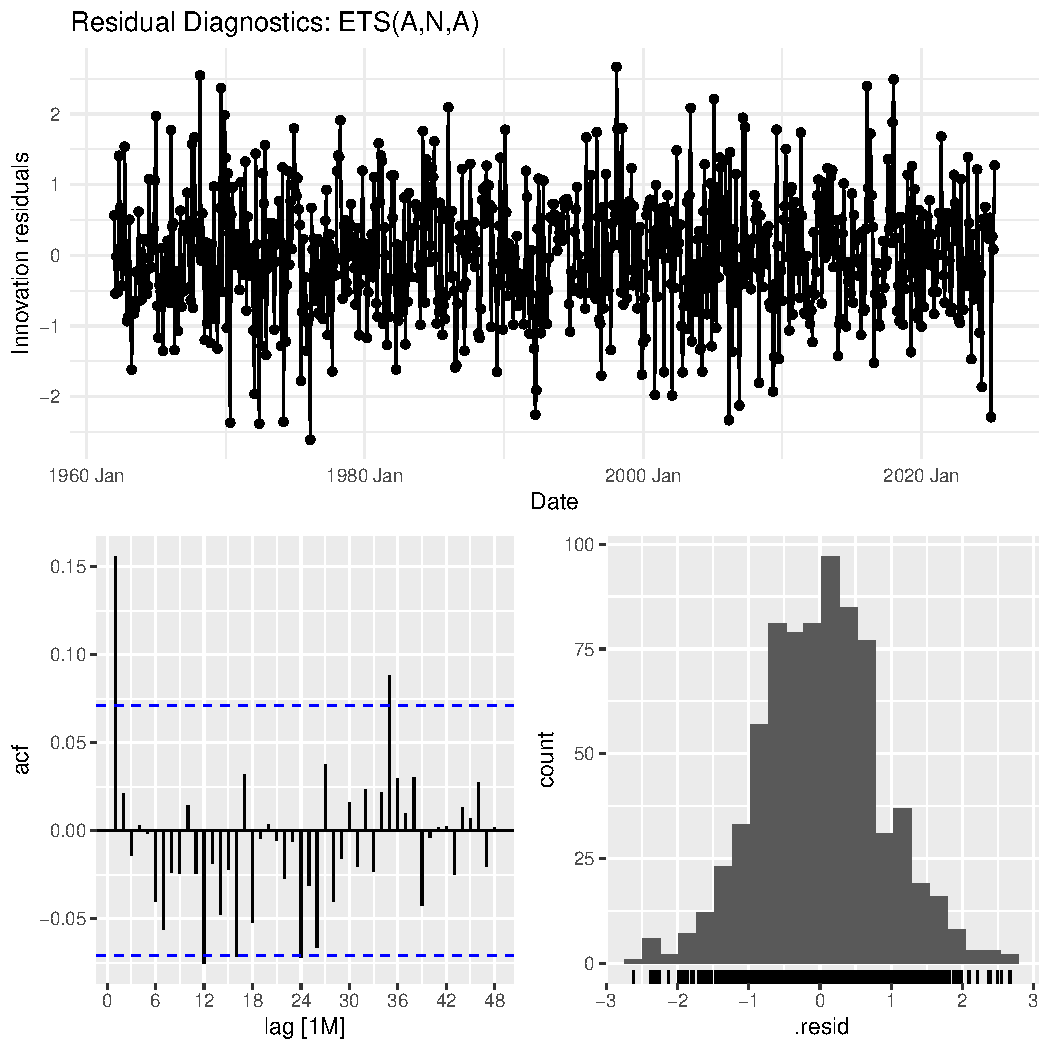
\includegraphics[width=1\linewidth]{figure/ets-assumptions-1} 

}

\caption[Residual Diagnostics for ETS(A,N,A) Model]{Residual Diagnostics for ETS(A,N,A) Model}\label{fig:ets-assumptions}
\end{figure}

\begin{kframe}\begin{alltt}
\hlcom{# Ljung-Box test}
\hlkwd{augment}\hldef{(best_fit)} \hlopt{%>%}
  \hlkwd{features}\hldef{(.innov, ljung_box,} \hlkwc{lag} \hldef{=} \hlnum{48}\hldef{,} \hlkwc{dof} \hldef{=} \hlnum{15}\hldef{)}
\end{alltt}
\begin{verbatim}
## # A tibble: 1 x 3
##   .model lb_stat lb_pvalue
##   <chr>    <dbl>     <dbl>
## 1 ANA       62.0   0.00163
\end{verbatim}
\end{kframe}
\end{knitrout}

The innovation residuals appear to fluctuate randomly around zero with roughly constant variance across the full time period, suggesting no obvious pattern or heteroscedasticity remains.

There are a few significant spikes, notably around lag 12 and lag 35, suggesting some remaining autocorrelation at seasonal lags that the model has not fully captured.

The residuals are roughly bell-shaped and centred near zero, which is broadly consistent with the normality assumption, though there is a slight right skew.

The Ljung-Box test shows with a test statistic of 62.03 and a p-value of 0.0016 < 0.05, we reject the null hypothesis of no autocorrelation in the residuals. This indicates statistically significant autocorrelation remains.

Based on the Ljung-Box result and the significant ACF spikes at seasonal lags, the ETS(A,N,A) model residuals are not fully consistent with white noise. This suggests the model may not have captured all the structure in the data, and therefore some caution is warranted when using this model for forecasting. Prediction intervals in particular may be underestimated.

\subsection{ARIMA Models Assumptions}

\begin{knitrout}
\definecolor{shadecolor}{rgb}{0.969, 0.969, 0.969}\color{fgcolor}\begin{kframe}
\begin{alltt}
\hlcom{# 4. Residual Diagnostics}

\hlkwd{augment}\hldef{(best_arima)} \hlopt{%>%}
  \hlkwd{features}\hldef{(.innov, ljung_box,} \hlkwc{lag} \hldef{=} \hlnum{24}\hldef{,} \hlkwc{dof} \hldef{=} \hlnum{3}\hldef{)}
\end{alltt}
\begin{verbatim}
## # A tibble: 1 x 3
##   .model   lb_stat lb_pvalue
##   <chr>      <dbl>     <dbl>
## 1 manual_2    50.5  0.000310
\end{verbatim}
\end{kframe}
\end{knitrout}

When evaluating the time plot of the innovation residuals, we observe that the series fluctuates around the zero mark, which indicates the errors have a zero mean. While the overall vertical spread of the errors appears roughly constant—suggesting we have met the constant variance assumption—there is a distinct, repeating pattern of clustering across the timeline. This predictable recurring pattern violates the white noise assumption, indicating that the model has failed to capture all the information, likely missing a seasonal or cyclic component that has been left behind in the residuals

ACF Plot of Residuals When examining the ACF plot, we observe five significant spikes poking outside the dashed blue boundary lines.For a white noise series, we would expect approximately 95\% of the autocorrelation spikes to sit safely inside these bounds. Because multiple spikes fall outside the lines, the residuals are significantly correlated across time, which violates the core assumption of white noise. This indicates that there is still predictable information left over that our ARIMA model failed to capture, and we should follow up with a Ljung-Box test to formally evaluate the autocorrelations as a collective group

Histogram of Residuals When evaluating the .resid histogram for our forecasting model, we observe a symmetric, bell-shaped distribution that is centered at exactly zero. Zero Mean: The center of the distribution at zero indicates that our model's residuals have a zero mean. This confirms that our forecasts are not biased; on average, the forecast errors cancel each other out, meaning the model does not systematically over-forecast or under-forecast the data.Normally Distributed: The symmetric bell shape confirms that the residuals are normally distributed. This shape shows that large forecast errors are rare, and smaller errors occur with equal frequency in both the positive and negative directions.
Prediction Intervals: Because we have confirmed that our residuals are normally distributed, we can safely rely on the mathematical calculations used to generate our prediction intervals. The symmetric, bell-shaped distribution centred near zero is consistent with the normality assumption, suggesting that the 95\% prediction intervals derived from this model are reliable.

\subsection{Dynamic Regression Models Assumptions}

\begin{knitrout}
\definecolor{shadecolor}{rgb}{0.969, 0.969, 0.969}\color{fgcolor}\begin{kframe}
\begin{alltt}
\hlcom{# Residual diagnostic plots for regression model}
\hldef{best_dynamic} \hlopt{%>%} \hlkwd{gg_tsresiduals}\hldef{()} \hlopt{+}
  \hlkwd{labs}\hldef{(}\hlkwc{title} \hldef{=} \hlsng{"Residual Diagnostics: Best Dynamic Regression Model (K=3)"}\hldef{)}
\end{alltt}
\end{kframe}\begin{figure}[H]

{\centering 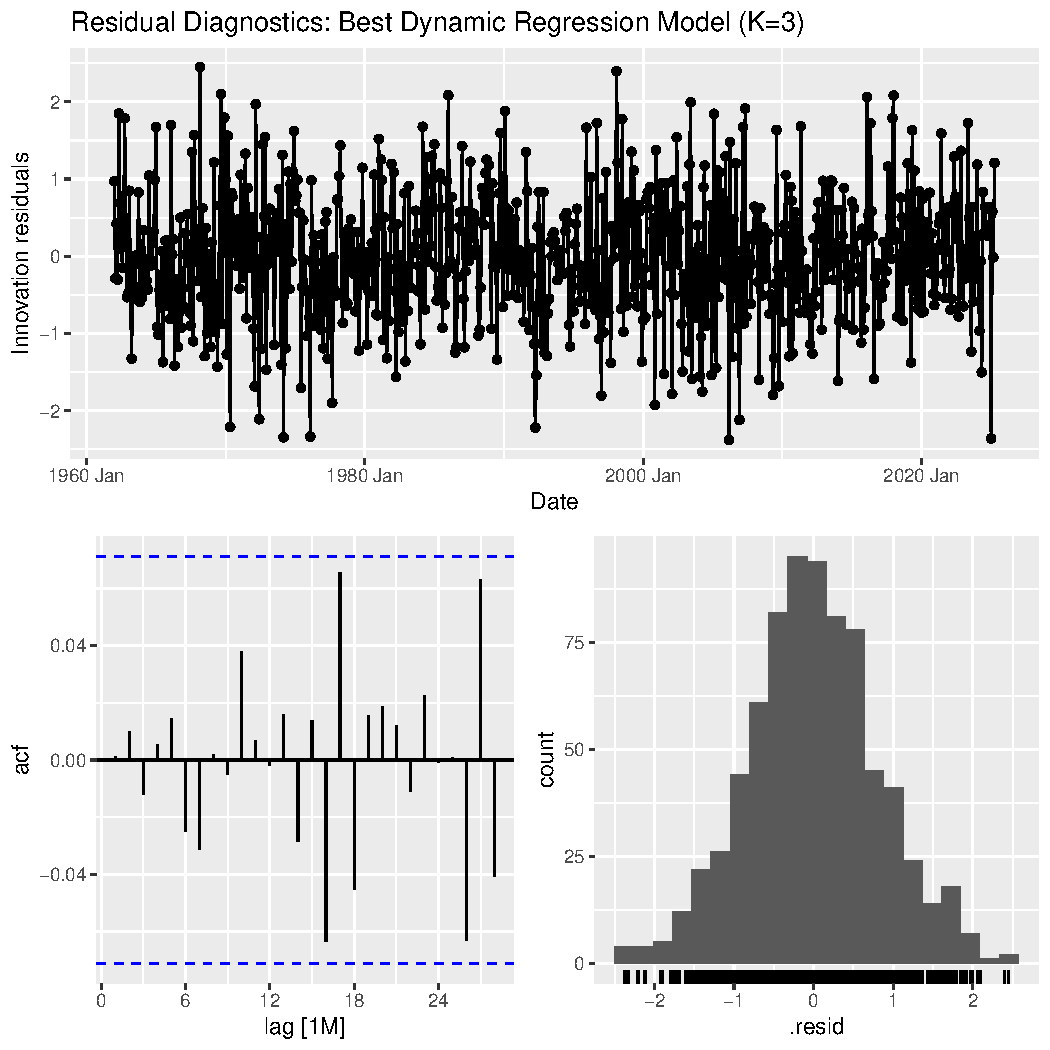
\includegraphics[width=1\linewidth]{figure/assumption-checking-1} 

}

\caption[Residual Diagnostics for the K=3 Dynamic Regression Model]{Residual Diagnostics for the K=3 Dynamic Regression Model}\label{fig:assumption-checking}
\end{figure}

\begin{kframe}\begin{alltt}
\hlcom{# Ljung-Box test to check remaining autocorrelation -> using lag = 24 for monthly data}
\hlkwd{augment}\hldef{(best_dynamic)} \hlopt{%>%}
  \hlkwd{features}\hldef{(.innov, ljung_box,} \hlkwc{lag} \hldef{=} \hlnum{24}\hldef{,} \hlkwc{dof} \hldef{=} \hlnum{5}\hldef{)}
\end{alltt}
\begin{verbatim}
## # A tibble: 1 x 3
##   .model lb_stat lb_pvalue
##   <chr>    <dbl>     <dbl>
## 1 K3        12.9     0.842
\end{verbatim}
\end{kframe}
\end{knitrout}

\textbf{Assumption Diagnostics} \\
For the model to be trusted for forecasting, the residuals must resemble independent white noise. Visual inspection of the innovation residuals shows constant variance over time with no obvious patterns. Furthermore, the ACF plot displays no significant autocorrelation spikes extending beyond the 95\% confidence bounds. This visual assessment is formally confirmed by the Ljung-Box test, which yielded a p-value of 0.842. Because the p-value is significantly greater than 0.05, we fail to reject the null hypothesis, confirming the residuals are indistinguishable from white noise. The K=3 dynamic regression model successfully captures all available time-dependent information and is highly trusted for forecasting.

\section{Forecasting}

\subsection{ETS Models Forecasting}

\begin{knitrout}
\definecolor{shadecolor}{rgb}{0.969, 0.969, 0.969}\color{fgcolor}\begin{kframe}
\begin{alltt}
\hldef{fc} \hlkwb{<-} \hldef{best_fit} \hlopt{%>%}
  \hlkwd{forecast}\hldef{(}\hlkwc{h} \hldef{=} \hlnum{12}\hldef{)}

\hlcom{# Accuracy on test set}
\hldef{fc} \hlopt{%>%}
  \hlkwd{accuracy}\hldef{(data)} \hlopt{%>%}
  \hlkwd{select}\hldef{(.model, RMSE, MAE, MAPE, MASE)} \hlopt{%>%}
  \hlkwd{arrange}\hldef{(RMSE)}
\end{alltt}
\begin{verbatim}
## # A tibble: 1 x 5
##   .model  RMSE   MAE  MAPE  MASE
##   <chr>  <dbl> <dbl> <dbl> <dbl>
## 1 ANA    0.748 0.637  4.45 0.649
\end{verbatim}
\begin{alltt}
\hlcom{# Plot forecasts vs actuals}
\hldef{fc} \hlopt{%>%}
  \hlkwd{autoplot}\hldef{(}
    \hldef{data} \hlopt{%>%} \hlkwd{filter}\hldef{(Date} \hlopt{>=} \hlkwd{yearmonth}\hldef{(}\hlsng{"2022 Jan"}\hldef{)),}
    \hlkwc{level} \hldef{=} \hlkwd{c}\hldef{(}\hlnum{80}\hldef{,} \hlnum{95}\hldef{),}
    \hlkwc{alpha} \hldef{=} \hlnum{0.5}
  \hldef{)} \hlopt{+}
  \hlkwd{labs}\hldef{(}\hlkwc{title} \hldef{=} \hlsng{"ETS Model Forecasts vs Actuals"}\hldef{,}
       \hlkwc{y} \hldef{=} \hlsng{"Temperature (°C)"}\hldef{,} \hlkwc{x} \hldef{=} \hlsng{"Date"}\hldef{)} \hlopt{+}
  \hlkwd{theme_minimal}\hldef{()}
\end{alltt}
\end{kframe}\begin{figure}[H]

{\centering 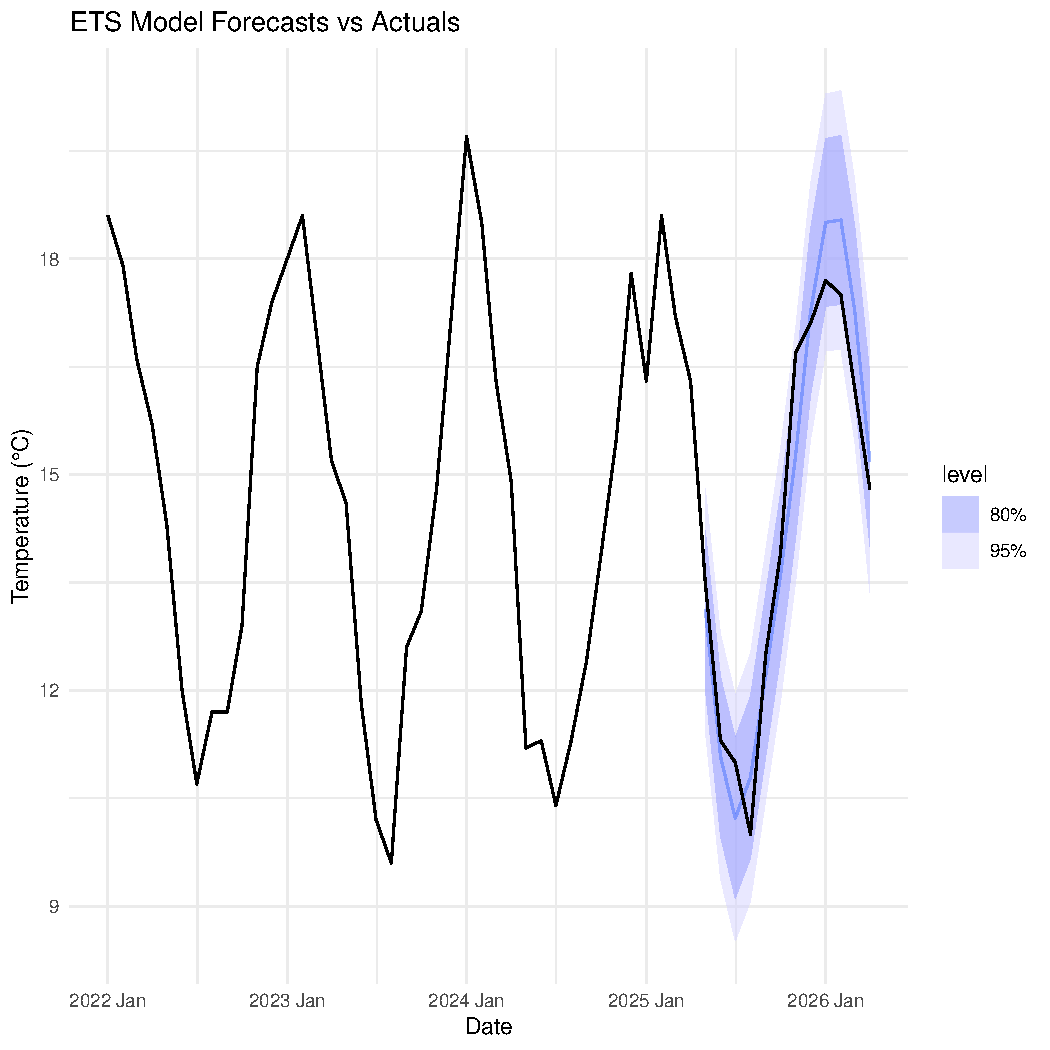
\includegraphics[width=1\linewidth]{figure/ets-forecasting-1} 

}

\caption[ETS Model Forecasts vs Actuals]{ETS Model Forecasts vs Actuals}\label{fig:ets-forecasting}
\end{figure}

\end{knitrout}

The ETS(A,N,A) model captures the seasonal pattern of Wellington temperatures well, with the point forecasts (black line) tracking the actual test set values closely. The actual observations fall well within the 95\% prediction interval throughout the forecast horizon, suggesting the model's uncertainty quantification is reasonable.

The model achieved an RMSE of 0.748 and MAE of 0.637, meaning forecasts were off by less than 1°C on average. The MAPE of 4.45\% indicates the model erred by around 4–5\% relative to actual values, and a MASE of 0.649 < 1 confirms the model outperforms a naive seasonal benchmark.

Despite the Ljung-Box test indicating some remaining autocorrelation in the residuals, the ETS(A,N,A) model performs reasonably well on the test set. The seasonal pattern is well captured, and the prediction intervals are neither too narrow nor too wide. However, the residual autocorrelation suggests there may be structure the model is missing.

\subsection{ARIMA Models Forecasting}

\begin{knitrout}
\definecolor{shadecolor}{rgb}{0.969, 0.969, 0.969}\color{fgcolor}\begin{kframe}
\begin{alltt}
\hlcom{# 5. Forecasting and Test Set Evaluation}

\hldef{forecast_arima} \hlkwb{<-} \hldef{best_arima} \hlopt{%>%}
  \hlkwd{forecast}\hldef{(}\hlkwc{h} \hldef{=} \hlnum{12}\hldef{)}

\hlcom{# Test set accuracy — pass full data for correct MASE}
\hldef{forecast_arima} \hlopt{%>%}
  \hlkwd{accuracy}\hldef{(data)} \hlopt{%>%}
  \hlkwd{select}\hldef{(.model, RMSE, MAE, MAPE, MASE)}
\end{alltt}
\begin{verbatim}
## # A tibble: 1 x 5
##   .model    RMSE   MAE  MAPE  MASE
##   <chr>    <dbl> <dbl> <dbl> <dbl>
## 1 manual_2 0.690 0.576  4.07 0.586
\end{verbatim}
\begin{alltt}
\hlcom{# Plot forecast against recent data}
\hldef{forecast_arima} \hlopt{%>%}
  \hlkwd{autoplot}\hldef{(}
    \hldef{data} \hlopt{%>%} \hlkwd{filter}\hldef{(Date} \hlopt{>=} \hlkwd{yearmonth}\hldef{(}\hlsng{"2022 Jan"}\hldef{)),}
    \hlkwc{level} \hldef{=} \hlkwd{c}\hldef{(}\hlnum{80}\hldef{,} \hlnum{95}\hldef{),}
    \hlkwc{alpha} \hldef{=} \hlnum{0.5}
  \hldef{)} \hlopt{+}
  \hlkwd{labs}\hldef{(}\hlkwc{title} \hldef{=} \hlsng{"ARIMA(1,0,0)(0,1,1) Forecast vs Actuals"}\hldef{,}
       \hlkwc{y} \hldef{=} \hlsng{"Temperature (°C)"}\hldef{,} \hlkwc{x} \hldef{=} \hlsng{"Date"}\hldef{)} \hlopt{+}
  \hlkwd{theme_minimal}\hldef{()}
\end{alltt}
\end{kframe}\begin{figure}[H]

{\centering 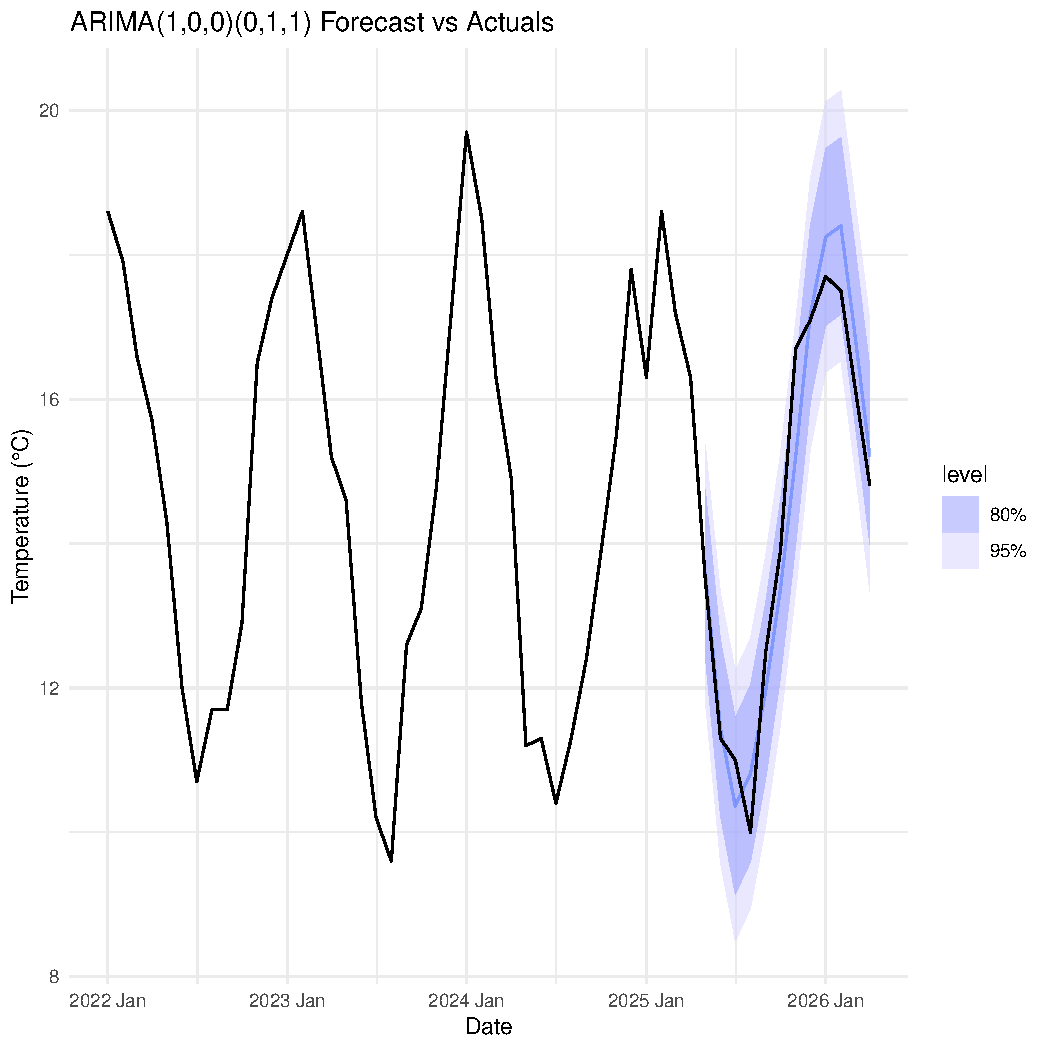
\includegraphics[width=1\linewidth]{figure/arima-forecasting-1} 

}

\caption[ARIMA Model Forecast vs Actuals]{ARIMA Model Forecast vs Actuals}\label{fig:arima-forecasting}
\end{figure}

\end{knitrout}

The ARIMA(1,0,0)(0,1,1) model with drift produces well-calibrated forecasts over the 12-month test horizon from May 2025 to April 2026. The point forecasts closely track the actual observed temperatures, correctly capturing both the summer peak and winter trough of the seasonal cycle. All actual observations fall comfortably within the 95\% prediction interval throughout the forecast horizon, indicating the model's uncertainty quantification is appropriate.

The model achieved an RMSE of 0.690 and MAE of 0.576, meaning forecasts were on average within 0.58°C of the actual values. The MAPE of 4.07\% confirms errors are small relative to the magnitude of Wellington temperatures, and a MASE of 0.586 demonstrates the model outperforms a seasonal naïve benchmark by approximately 41\%.

The prediction interval is notably narrow, remaining within roughly +-1.5°C for most of the forecast horizon, which reflects the high regularity of Wellington's seasonal temperature cycle and the model's confidence in its seasonal pattern.

\subsection{Dynamic Regression Models Forecasting}

\begin{knitrout}
\definecolor{shadecolor}{rgb}{0.969, 0.969, 0.969}\color{fgcolor}\begin{kframe}
\begin{alltt}
\hlcom{# Produce point forecasts and prediction intervals for h = 12 months}
\hlcom{# Can add ETS and ARIMA models to the pipeline alongside best_dynamic}
\hldef{forecasts} \hlkwb{<-} \hldef{best_dynamic} \hlopt{%>%}
  \hlkwd{forecast}\hldef{(}\hlkwc{h}\hldef{=}\hlnum{12}\hldef{)}

\hlcom{# compare forecast errors on test set}
\hlkwd{accuracy}\hldef{(forecasts, data)} \hlopt{%>%}
  \hlkwd{select}\hldef{(.model, .type, RMSE, MAE, MAPE, MASE)} \hlopt{%>%}
  \hlkwd{arrange}\hldef{(RMSE)}
\end{alltt}
\begin{verbatim}
## # A tibble: 1 x 6
##   .model .type  RMSE   MAE  MAPE  MASE
##   <chr>  <chr> <dbl> <dbl> <dbl> <dbl>
## 1 K3     Test  0.759 0.647  4.56 0.659
\end{verbatim}
\begin{alltt}
\hlcom{# plotting forecasts against test set ("zoomed" in for visibility)}
\hldef{forecasts} \hlopt{%>%}
  \hlcom{# Filtering training data to only show recent years (e.g., 2023 onwards)}
  \hlkwd{autoplot}\hldef{(data} \hlopt{%>%} \hlkwd{filter}\hldef{(Date} \hlopt{>=} \hlkwd{yearmonth}\hldef{(}\hlsng{"2023 Jan"}\hldef{)),} \hlkwc{level} \hldef{=} \hlkwd{c}\hldef{(}\hlnum{80}\hldef{,} \hlnum{95}\hldef{))} \hlopt{+}
  \hlkwd{autolayer}\hldef{(test, Temperature,} \hlkwc{color} \hldef{=} \hlsng{"black"}\hldef{,} \hlkwc{linewidth} \hldef{=} \hlnum{0.8}\hldef{)} \hlopt{+}
  \hlkwd{labs}\hldef{(}\hlkwc{title} \hldef{=} \hlsng{"Wellington Monthly Temperature Forecast vs Actuals"}\hldef{,}
       \hlkwc{subtitle} \hldef{=} \hlsng{"Zoomed View: Jan 2023 - April 2026"}\hldef{,}
       \hlkwc{y} \hldef{=} \hlsng{"Temperature (C)"}\hldef{,}
       \hlkwc{x} \hldef{=} \hlsng{"Date"}\hldef{)} \hlopt{+}
  \hlkwd{theme_minimal}\hldef{()}
\end{alltt}
\end{kframe}\begin{figure}[H]

{\centering 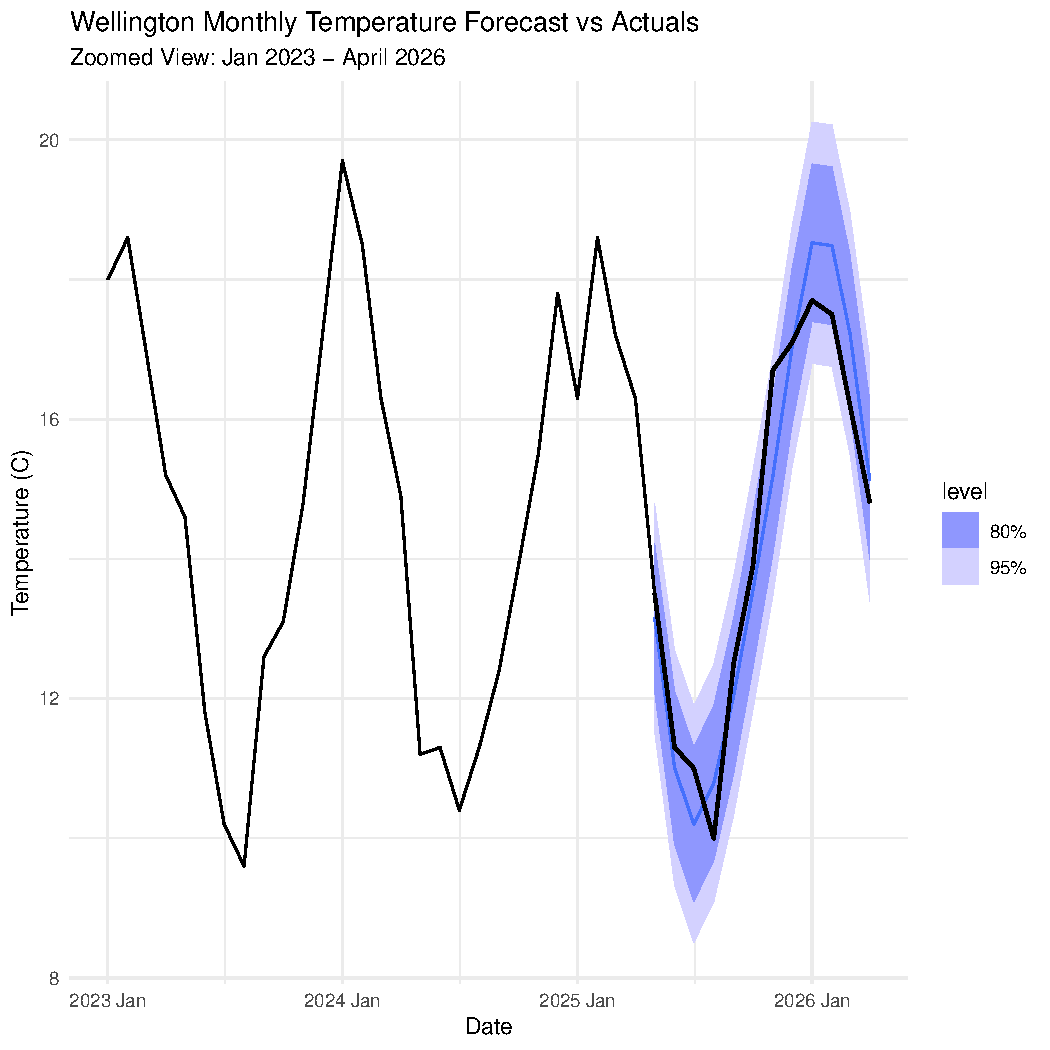
\includegraphics[width=1\linewidth]{figure/forecasting-1} 

}

\caption[Wellington Temperature Forecast]{Wellington Temperature Forecast}\label{fig:forecasting}
\end{figure}

\end{knitrout}

\subsection{Forecast Comparison}

\begin{knitrout}
\definecolor{shadecolor}{rgb}{0.969, 0.969, 0.969}\color{fgcolor}\begin{kframe}
\begin{alltt}
\hlcom{# Combine all three best models and forecast together}
\hldef{fit_all} \hlkwb{<-} \hldef{training} \hlopt{%>%}
  \hlkwd{model}\hldef{(}
    \hlkwc{ETS}     \hldef{=} \hlkwd{ETS}\hldef{(Temperature} \hlopt{~} \hlkwd{error}\hldef{(}\hlsng{"A"}\hldef{)} \hlopt{+} \hlkwd{trend}\hldef{(}\hlsng{"N"}\hldef{)} \hlopt{+} \hlkwd{season}\hldef{(}\hlsng{"A"}\hldef{)),}
    \hlkwc{ARIMA}   \hldef{=} \hlkwd{ARIMA}\hldef{(Temperature} \hlopt{~} \hlkwd{pdq}\hldef{(}\hlnum{1}\hldef{,}\hlnum{0}\hldef{,}\hlnum{0}\hldef{)} \hlopt{+} \hlkwd{PDQ}\hldef{(}\hlnum{0}\hldef{,}\hlnum{1}\hldef{,}\hlnum{1}\hldef{)),}
    \hlkwc{Dynamic} \hldef{=} \hlkwd{ARIMA}\hldef{(Temperature} \hlopt{~} \hlkwd{trend}\hldef{()} \hlopt{+} \hlkwd{fourier}\hldef{(}\hlkwc{K} \hldef{=} \hlnum{3}\hldef{))}
  \hldef{)}

\hldef{fc_all} \hlkwb{<-} \hldef{fit_all} \hlopt{%>%} \hlkwd{forecast}\hldef{(}\hlkwc{h} \hldef{=} \hlnum{12}\hldef{)}

\hlcom{# Combined accuracy table}
\hldef{fc_all} \hlopt{%>%}
  \hlkwd{accuracy}\hldef{(data)} \hlopt{%>%}
  \hlkwd{select}\hldef{(.model, RMSE, MAE, MAPE, MASE)} \hlopt{%>%}
  \hlkwd{arrange}\hldef{(RMSE)}
\end{alltt}
\begin{verbatim}
## # A tibble: 3 x 5
##   .model   RMSE   MAE  MAPE  MASE
##   <chr>   <dbl> <dbl> <dbl> <dbl>
## 1 ARIMA   0.690 0.576  4.07 0.586
## 2 ETS     0.748 0.637  4.45 0.649
## 3 Dynamic 0.759 0.647  4.56 0.659
\end{verbatim}
\begin{alltt}
\hlcom{# Combined plot}
\hldef{fc_all} \hlopt{%>%}
  \hlkwd{autoplot}\hldef{(}
    \hldef{data} \hlopt{%>%} \hlkwd{filter}\hldef{(Date} \hlopt{>=} \hlkwd{yearmonth}\hldef{(}\hlsng{"2022 Jan"}\hldef{)),}
    \hlkwc{level} \hldef{=} \hlkwd{c}\hldef{(}\hlnum{80}\hldef{,} \hlnum{95}\hldef{),}
    \hlkwc{alpha} \hldef{=} \hlnum{0.4}
  \hldef{)} \hlopt{+}
  \hlkwd{autolayer}\hldef{(test, Temperature,} \hlkwc{colour} \hldef{=} \hlsng{"black"}\hldef{,} \hlkwc{linewidth} \hldef{=} \hlnum{0.8}\hldef{)} \hlopt{+}
  \hlkwd{labs}\hldef{(}\hlkwc{title} \hldef{=} \hlsng{"Wellington Temperature: All Model Forecasts vs Actuals"}\hldef{,}
       \hlkwc{subtitle} \hldef{=} \hlsng{"May 2025 - April 2026 (h = 12)"}\hldef{,}
       \hlkwc{y} \hldef{=} \hlsng{"Temperature (\textbackslash{}u00b0C)"}\hldef{,} \hlkwc{x} \hldef{=} \hlsng{"Date"}\hldef{)} \hlopt{+}
  \hlkwd{theme_minimal}\hldef{()}
\end{alltt}
\end{kframe}\begin{figure}[H]

{\centering 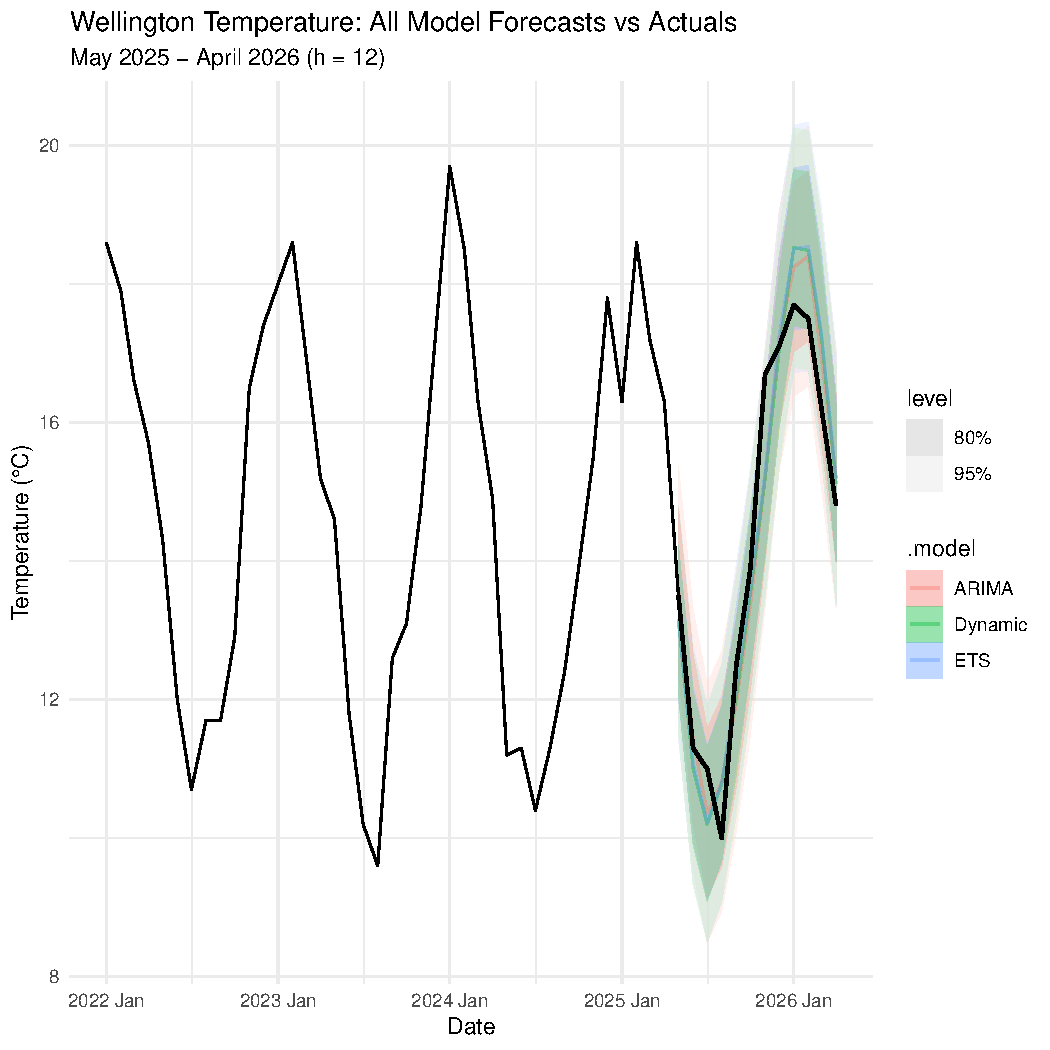
\includegraphics[width=1\linewidth]{figure/forecasting-combined-1} 

}

\caption[Combined Forecasts vs Actuals]{Combined Forecasts vs Actuals: All Three Models}\label{fig:forecasting-combined}
\end{figure}

\end{knitrout}

All three models produced reasonable forecasts, successfully capturing 
Wellington's strong seasonal cycle over the 12-month test horizon. 
However, the models differ meaningfully in their accuracy and 
assumption satisfaction.

The ARIMA(1,0,0)(0,1,1) with drift was the best performing 
model across all metrics, achieving an RMSE of 0.690 and MASE of 0.586. 
This represents approximately a 41\% improvement over a seasonal 
naive benchmark. The inclusion of an AR(1) term allowed the model 
to capture short-term autocorrelation that the ETS model left unmodelled, 
and the drift term accounted for the slow warming trend identified in 
the STL decomposition. Residual diagnostics, however, indicated the 
Ljung-Box test rejected white noise ($p = 0.00031$), suggesting some 
remaining structure.

The ETS(A,N,A) model performed competitively, achieving an RMSE of 
0.748 and MASE of 0.649, only marginally worse than the ARIMA model. 
This is consistent with the theoretical equivalence between ETS(A,N,A) 
and ARIMA(0,1,1)(0,1,1); the two models capture similar 
dynamics, with the primary difference being the AR(1) term in the 
winning ARIMA specification. The ETS model also failed the Ljung-Box 
test ($p = 0.0016$), indicating residual autocorrelation.

The Dynamic Regression model (K=3) performed weakest on the test set 
with an RMSE of 0.759 and MASE of 0.659, despite having the best 
residual diagnostics of all three models, the only model whose 
residuals passed the Ljung-Box test ($p = 0.842$). This illustrates 
an important caveat: a well-specified model in-sample does not 
guarantee the best out-of-sample performance. The Fourier terms 
impose a fixed seasonal structure that may be less adaptive than the 
data-driven seasonal updating in ETS and ARIMA. Additionally, the 
dynamic regression's wider prediction intervals (showing both 80\% 
and 95\% bands) reflect greater uncertainty, though all actual 
observations remained within the 95\% bounds.

Overall, the ARIMA model is recommended as the primary forecasting 
tool for Wellington monthly temperatures, with the ETS model as a 
close and computationally simpler alternative.

\section{LLMs in Time Series Analysis}



\section{Member Contributions}

\begin{itemize}
    \item \textbf{[Eric]:} Completed Sections 
    \item \textbf{[Simon]:} Completed Sections
    \item \textbf{[Dominicus]:} Completed Sections
\end{itemize}

\end{document}
